\section{Projektbudget}

Das Projektbudget bezieht sich auf die vorgesehenen Arbeitsstunden. Die Projektmanagement-Stunden werden mit 148 Sfr. verrechnet, die restlichen mit 74 SFr. In Abbildung \ref{fig::Budget_1} wird die Kostenaufstellung gezeigt und in Abbildung \ref{fig::Budget_2} die Kostenverteilung.


\begin{figure}[h] 
\centering
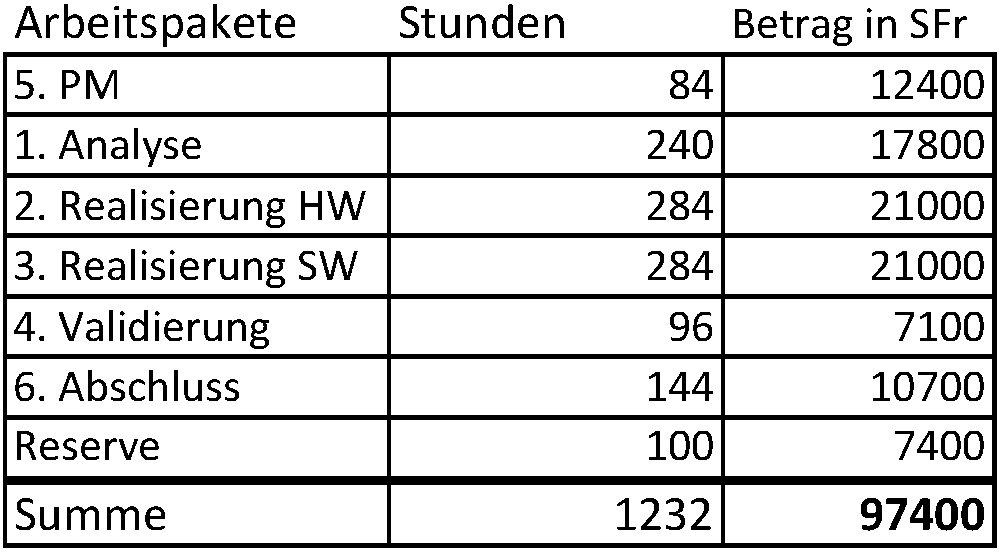
\includegraphics[width=0.6\textwidth]{Budget_1.png}%
\caption{Kostenaufstellung}%
\label{fig::Budget_1}%
\end{figure}

\begin{figure}[h] 
\centering
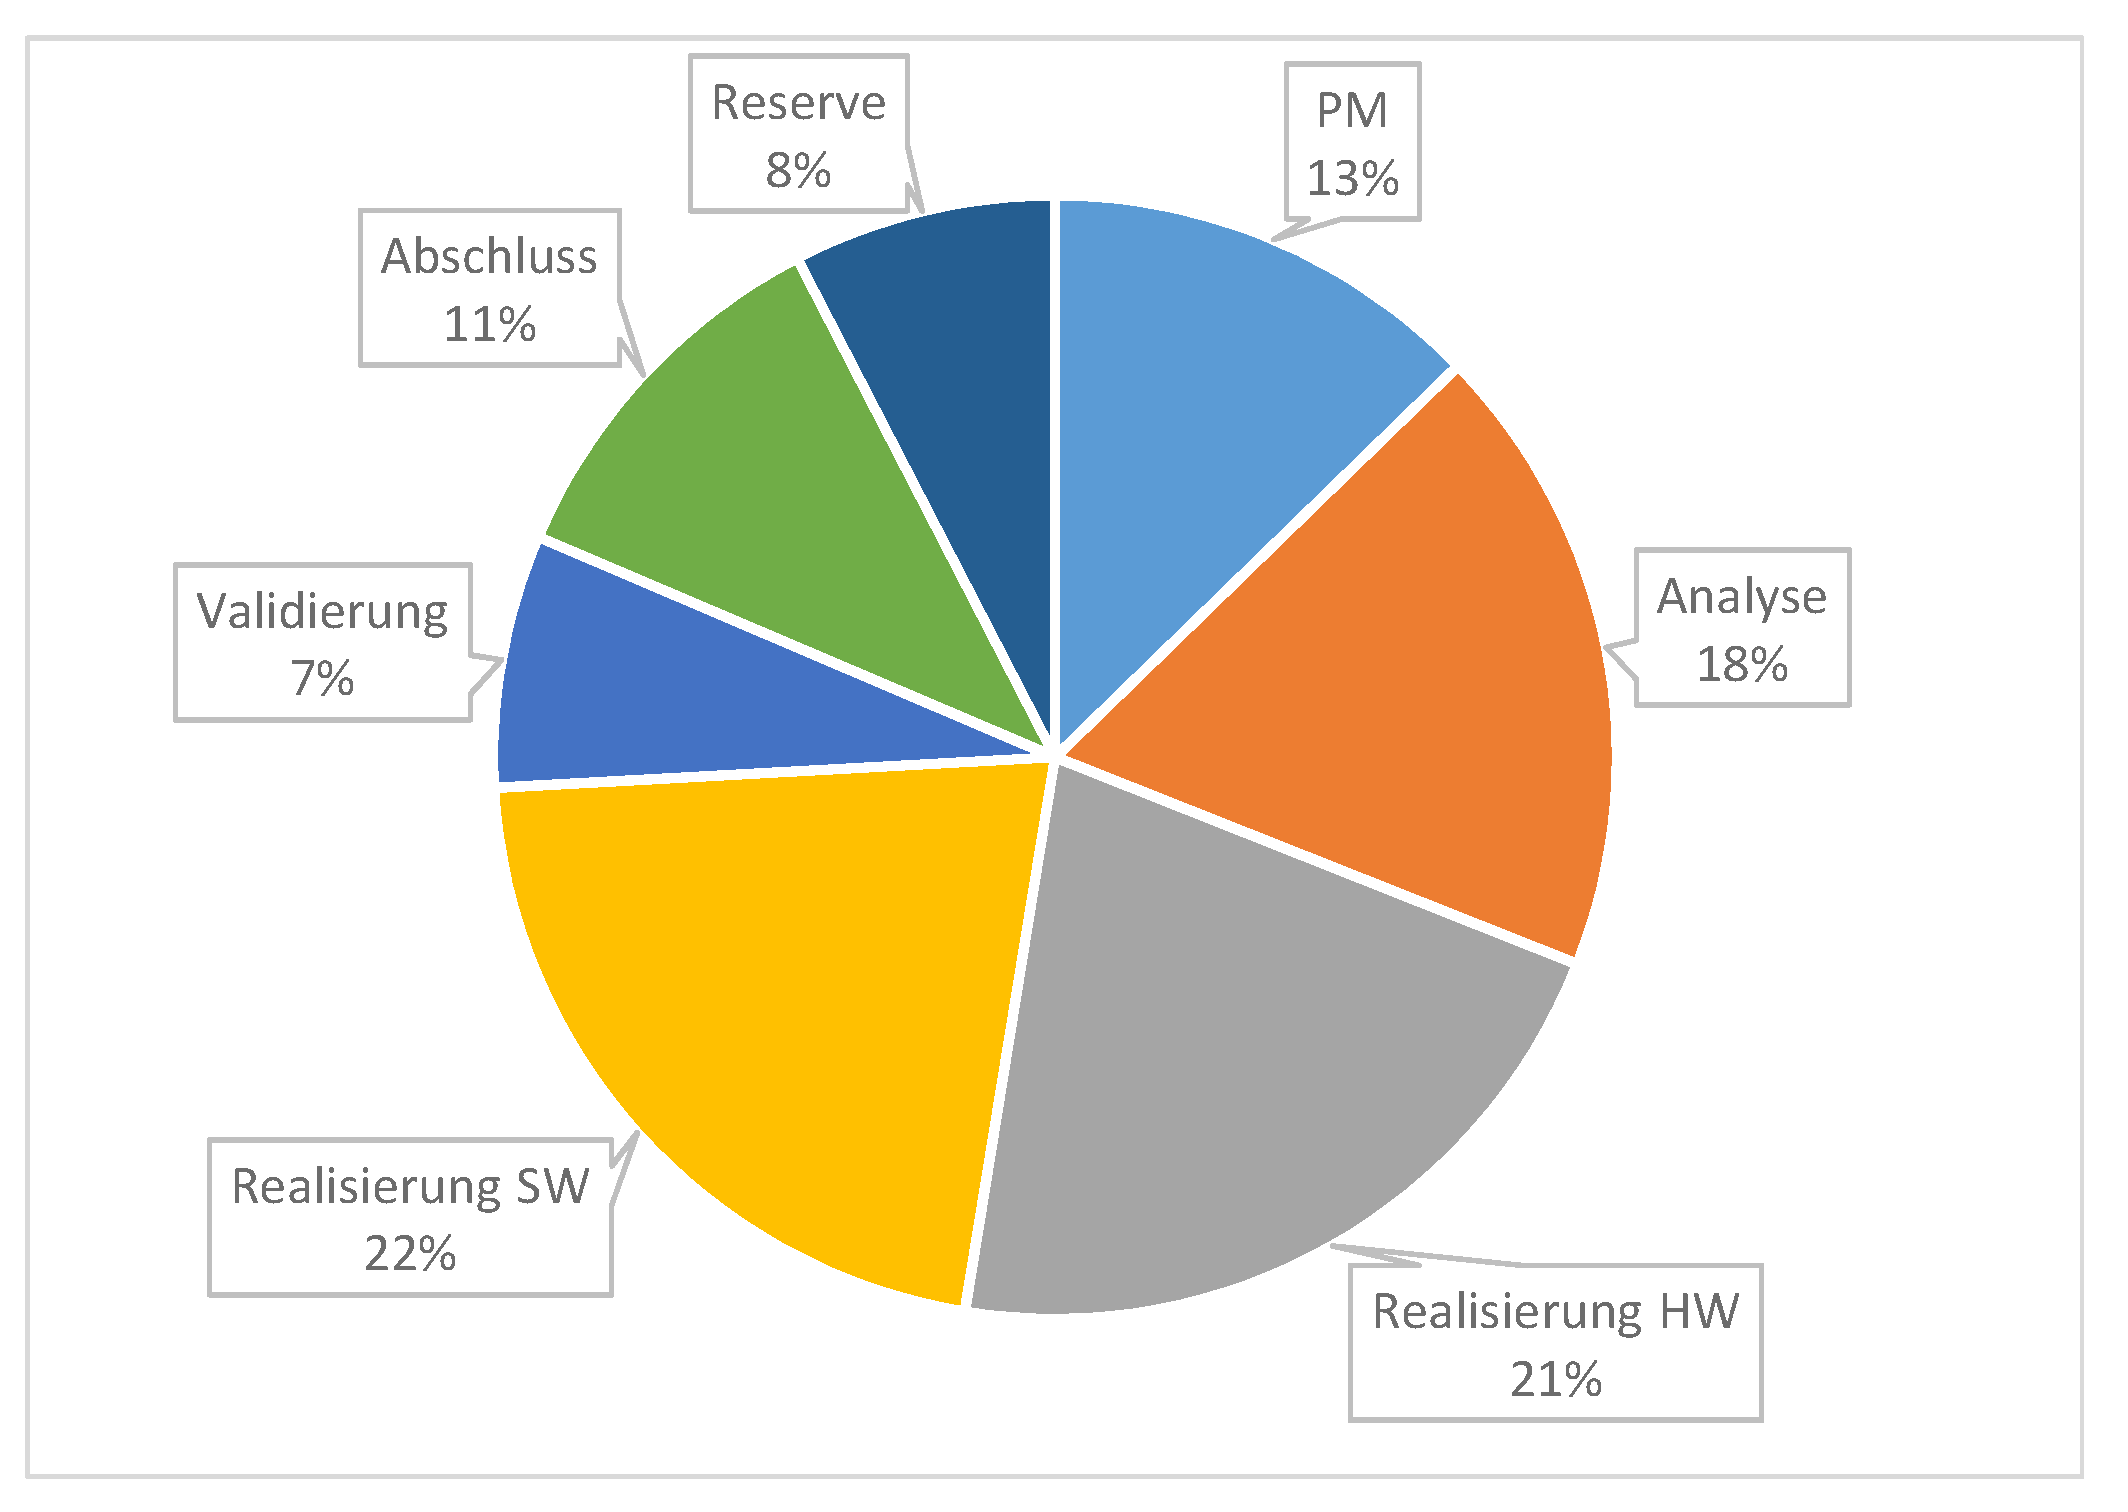
\includegraphics[width=0.8\textwidth]{Budget_2.png}%
\caption{Kostenverteilung}%
\label{fig::Budget_2}%
\end{figure}

Die Materialkosten können zu diesem Zeitpunkt noch nicht abgeschätzt werden, jedoch sollte das maximale Budget für den Materialeinkauf von 250 Franken nicht überschritten werden.